\documentclass[11pt]{article}

% Packages for Latex document
\usepackage[utf8]{inputenc}

% Used for expanding text space
\usepackage[a4paper, margin=20mm]{geometry}

% Used for \mathbb{} function
\usepackage{amssymb}

% Used for \text{} function
\usepackage{amsmath}

% Used for writing algorithms
\usepackage{algorithm}
\usepackage{algorithmic}

% For making code presentable
\usepackage{listings}
\usepackage{xcolor}

% For graphics
\usepackage{graphicx}

% New colors defined below
\definecolor{codegreen}{rgb}{0,0.6,0}
\definecolor{codegray}{rgb}{0.5,0.5,0.5}
\definecolor{codepurple}{rgb}{0.58,0,0.82}
\definecolor{backcolour}{rgb}{0.95,0.95,0.92}

% Code listing style named "mystyle"
\lstdefinestyle{mystyle}{
  backgroundcolor=\color{backcolour}, commentstyle=\color{codegreen},
  keywordstyle=\color{magenta},
  numberstyle=\tiny\color{codegray},
  stringstyle=\color{codepurple},
  basicstyle=\ttfamily,
  breakatwhitespace=false,         
  breaklines=true,                 
  captionpos=b,                    
  keepspaces=true,                   
  numbersep=5pt,                  
  showspaces=false,                
  showstringspaces=false,
  showtabs=false,                  
  tabsize=2
}

% "mystyle" code listing set
\lstset{style=mystyle}

% Additional formatting
\setlength{\parindent}{0em}
\setlength{\parskip}{0em}

% Begin the document
\begin{document}

% Title card
\begin{titlepage}
    
    % Implement a title
    \title{Trading Strategy Back-Tester Creation\\
    \large A Tutorial on Creating a Custom\\ Trading Strategy Back-Testing Algorithm}
    
    
    % Implement the author
    \author{Ivan Silajev}
    
    % Use date section for extra info
    \date{
    % State organisation
    Warwick Coding Society \\
    % State e-mail of authors
    \texttt{ivan.silajev@warwick.ac.uk}
    }
    
    % Create the title section in PDF
    \maketitle
    
    % Implement the contents section
    \tableofcontents
    
\end{titlepage}

% Start introduction section
\section{Introduction}

% Introduction: 
% Sentence for stating what the document is about
% Checked!
This \textbf{Warwick Coding Society} report outlines the theory and the creation of a trading strategy back-testing algorithm using the Python programming language.
% Sentence for stating how the document presents the information
% Checked!
This document's approach to presenting the theory involves concisely explaining each topic before introducing the mathematics and Python code.
% Sentence stating that the document is a programming tutorial as well
% Checked!
We designed the code shown throughout the report to be flexible, so anyone who follows it to create their trading strategy back-tester would have an easier time changing it to their liking.\\

% List mentioning the most important topics the document
The topics covered in this report include:
\begin{itemize}
    \item What is \textbf{trading} and \textbf{arbitrage}?
    \item What is a \textbf{trading strategy} and how use it?
    \item What is \textbf{portfolio optimisation} and how it's done?
\end{itemize}

% Sentence for showing existing packages for back testing and portfolio optimisation
%The report will also cover existing back testing and portfolio optimisation Python packages like \textbf{Backtrader} and \textbf{PyPortfolioOpt}.\\

% Sentence explaining the motivation for writing the document
% Checked!
The motivation for creating this report is to introduce programmers of any skill level to algorithmic trading and back-testing in a clear, concise manner, in line with Warwick Coding Society's goal of \textbf{making programming accessible}.
% Sentence also mentioning collaborative intention behind document
% This report is also part of a collaboration project with the WFS Quant Finance Team.
% Sentence mentioning how collaborative aspect stands out
% This WCS report was made to perfectly complement the WFS report on 'trading strategy comparisons', as one can replicate the results in that report with the tools they learn in this one.

% Start trading basics section
\section{Trading Basics}

% Section on what is trading
\subsection{What is Trading?}

% A general definition of trading
\textbf{Trading} is the exchange of value between two entities.
% A general definition of a market
A \textbf{market} is a field where entities trade.
% Mention what the most active markets are with examples
% Checked!
The most active markets today comprise financial asset markets, including the \textbf{New York Stock Exchange (NYSE)} and the \textbf{National Association of Securities Dealers Automated Quotations (NASDAQ)}.\\

% Motivate the reason for focusing on financial markets only
% Checked!
Financial asset markets are ever-trending due to their increasing accessibility to the general public and the simplicity of trading on them.
% State that reason restricts document to financial markets only, though information is applicable to any market
% Checked!
For this reason, this report will be primarily focusing on financial asset markets, though the methodology presented here applies to any market.\\

% Give extra insight on past of algorithmic trading
% Checked!
With the progress of technology and mathematics in the late 20th century, companies like \textbf{Renaissance Technologies} investigated algorithmic trading strategies to automate and optimise their trading activity in financial asset markets.
% State that algorithmic trading is now accessible more than ever
% Checked!
Currently, anyone can access financial markets through the many internet brokers that exist, allowing anyone to use algorithmic trading methods to automate their trading activity.\\

% State there are two ways of profiting from financial asset trading
% Checked!
There are two common ways to profit from trading in financial asset markets.

% List trading profiting techniques
\begin{itemize}

    % Explain long trading
    % Checked!
    \item In a \textbf{buy/long position}, one buys an asset on the market at an agreed price and time. Then, they sell the asset on the market when it increases in price, thus profiting from the increase in the price.
    
    % Explain short trading
    % Checked!
    \item In a \textbf{sell/short position}, one borrows assets from the broker and sells them on the market at an agreed price and time. Then, they buy back the asset when it decreases in price and returns it to the broker, thus profiting from the decrease in the price.
    
\end{itemize}

% Point to extra resources for the curious
% Checked!
For more details on how brokers, financial markets, and assets work, the reader can resort to the resources mentioned in section 7 of this report.

\newpage

% Start section on arbitrage
\subsection{What is Arbitrage?}

% Give a definition of arbitrage
% Checked!
\textbf{Arbitrage} involves exploiting inefficiencies across markets to trade more profitably.
% Give a definition of arbitrage opportunity
% Checked!
An \textbf{arbitrage opportunity} is the potential of investing a net-zero worth of capital into assets and profiting from them without risk.
% Give a simpler definition of arbitrage opportunity that highlights its significance
% Checked!
Simply put, an arbitrage opportunity can give something from nothing with no risk of loss.\\

% Explain how can arbitrage opportunities be found
% Checked!
One can find arbitrage opportunities using data that accurately reflects the current demand for different assets, allowing them to predict which assets will be profitable.
% State the generality of arbitrage for markets
% Checked!
Again, arbitrage is a general concept applicable to any set of markets.\\

% List basic sources of arbitrage opportunity info sources
% State that there are more sources of arbitrage opportunity information
% Checked!
Standard arbitrage opportunity detection methods include multivariate trend analysis, internet social trend analysis and portfolio optimisation methods, like the one explained in section 4.4 of this report.

% Start section on trading strategy utilisation
\section{Trading Strategy Back-Testing Theory}

% Give a general definition of a trading strategy
% Checked!
A \textbf{trading strategy} is a rule for when and how to trade an asset over time.
\textbf{Back-testing} is the testing of a trading strategy's profitability with historical price data.
% State that trading strategies have a standard
We start by outlining what we expect from a trading strategy.

% Start section explaining what a good trading strategy is
\subsection{The Characteristics of a Good Trading Strategy}

% State the goal of trading
The aim of trade is to \textbf{profit}.
% Restate the different ways to trade on financial markets
One can trade in the financial market by opening long or short positions on financial assets.\\

% How to trade profitably with long positions
\textbf{Long positions} are profitable when assets are bought at low prices and sold at higher prices.
% How to trade profitably with short positions
\textbf{Short positions} are profitable when assets are sold at high prices and bought at lower prices.\\

% Summarise the properties of a profitable trading strategy
Therefore, a good trading strategy:
\begin{itemize}
    \item Opens and holds long positions while the asset price trends upwards
    \item Opens and holds short positions while the asset price trends downwards
    \item Closes long positions when the asset price starts trending downwards
    \item Closes short positions when the asset price starts trending upwards
\end{itemize}

% Create section for initial mathematical concepts
\subsubsection{Mathematical Preliminaries}

% Start with defining the time domain
Define the set of times for which the price data of a given asset is observed as the countable set $T \subset \mathbb{R}$.\\

% Define the four price series
Brokers and financial websites provide data on the historical prices of assets, including the close, open, low and high prices for different time intervals.
Define the close, open, low and high prices as follows:
\begin{itemize}
    \item Close price series: $P_{c}:T \mapsto \mathbb{R^{+}}$
    \item Open price series: $P_{o}:T \mapsto \mathbb{R^{+}}$
    \item Low price series: $P_{l}:T \mapsto \mathbb{R^{+}}$
    \item High price series: $P_{h}:T \mapsto \mathbb{R^{+}}$
\end{itemize}

These series can be used for the construction of \textbf{indicator series}. See section 6 of this report for an example.

% Introduce indicator series
\subsection{Indicator Series}

% State what type of information trading strategies require for being good
A trading strategy involves using information about the asset price trend.
% State the form in which this information exists in
This information is usually in the form of a time series, known as an \textbf{indicator series}, showing when the asset price is possibly increasing or decreasing. One can always transform price trend information not in the form of an indicator series to be one.\\

% Summarise what an indicator series represents
An indicator series is:
\begin{itemize}
    \item Positive when the price trends upwards
    \item Negative when the price trends downwards
    \item Zero when the price trend is stable
\end{itemize}

% Begin mathematical description of an indicator series
\subsubsection{Mathematical Description}


Define an indicator time series $I:T \mapsto \mathbb{R}$ as a function of time.\\

An example of a trivial indicator series is the difference between the close and open prices of the asset traded:
\begin{center}
    $I(t) = P_c(t) - P_o(t)$
\end{center}

Another example of a trivial indicator series involves using the first order difference of the closed prices:
\begin{center}
    $I(t) = P_c(t) - P_c(t - \Delta_t)$
\end{center}

Where $\Delta_t$ is the difference between time $t$ and the latest time before $t$ in set $T$, or, more precisely: 
\begin{center}
    $\Delta_t = t - \sup \left ( T \cap (\infty, t) \right )$
\end{center}

Deriving reliable indicators is a separate science in which quantitative traders specialise.
% The WFS report on trading strategy comparisons gives some insight into the most commonly used indicators to date.

\subsection{Trade Signal Series}

A \textbf{trade signal series} informs when a given trade type should be open according a given indicator series.\\

The long trade signal series is:
\begin{itemize}
    \item Equal to one when the indicator is strictly positive
    \item Equal to zero otherwise
\end{itemize}

The short trade signal series is:
\begin{itemize}
    \item Equal to one when the indicator is strictly negative
    \item Equal to zero otherwise
\end{itemize}

\subsubsection{Mathematical Description}

The \textbf{long trade signal series} $V_l:T \mapsto \{ 0,1 \}$ is defined as:
\begin{center}
    $V_l(t) = \text{sign}(\text{max}\{I(t),0 \})$
\end{center}

The \textbf{short trade signal series} $V_s(t)$ is trivially derived by changing the sign of the indicator.
\begin{center}
    $V_s(t) = \text{sign}(\text{max}\{-I(t),0 \})$
\end{center}

\subsection{Action Series}

An \textbf{action series} informs exactly when to open or close trades of a given type based on a given trade signal series.\\

The action series is:
\begin{itemize}
    \item Equal to one when the trade must be opened
    \item Equal to zero when the position must be held (inaction)
    \item Equal to minus one when the trade must be closed
\end{itemize}

\subsubsection{Mathematical Description}

The \textbf{action series} $A:T \mapsto \{ -1,0,1 \}$, for a given trade signal series $V(t)$, is defined as:
\begin{center}
    $A(t) = \begin{cases}
V(t) & \text{ if } t= \inf{T}\\ 
V(t) - V(t - \Delta_t) & \text{ if }  t > \inf{T}
\end{cases}$
\end{center}



\subsection{Alpha Series}

Finally, the \textbf{alpha series} shows the ratio of the value of the investment with its previous value at a given time under the use of a trading strategy.\\

When the trade is inactive, the alpha series will take the value one, since no capital is invested in the asset. When the trade is active, the alpha series will output the ratio change in the investment according to the close price series.\\

The alpha series of a given asset and trading strategy is what's used to evaluate the performance of the trading strategy for the asset.

\subsubsection{Mathematical Description}

The alpha series $\alpha : T \mapsto \mathbb{R}^{+}$, for a given trade signal series $V(t)$ and action series $A(t)$, is generated using the following algorithm:

\begin{algorithmic}[1]
\REQUIRE $T \wedge V(t) \wedge A(t) \wedge P_c(t) \wedge r$
\ENSURE $\alpha(t)$
\FOR{$t = \inf T$ \TO $\sup T$}
\IF{$A(t) = 1$}
\STATE $\alpha(t) \leftarrow 1$
\STATE $P_0 \leftarrow P_c(t)$
\ELSIF{$A(t) = 0$}
\IF{$V(t) = 0$}
\STATE $\alpha(t) \leftarrow 1$
\ELSIF{$V(t) = 1$}
\STATE $\alpha(t) \leftarrow (P_0 + r \cdot (P_c(t) - P_0))/(P_0 + r \cdot (P_c(t- \Delta_t) - P_0))$
\ENDIF
\ELSIF{$A(t) = -1$}
\STATE $\alpha(t) \leftarrow (P_0 + r \cdot (P_c(t) - P_0))/(P_0 + r \cdot (P_c(t- \Delta_t) - P_0))$
\ENDIF
\ENDFOR
\end{algorithmic}
The capital ratio $r$ is the proportion of capital dedicated to the trade. A positive $r$ generates an alpha series for a long position strategy. A negative $r$ generates an alpha series for a short position strategy.

\subsection{Back-Test of an Alpha Series}

Using the alpha series generating algorithm, one can generate the alpha series for a trading strategy consisting of:

\begin{itemize}
    \item Long positions only, giving the \textbf{long alpha series} $\alpha_l(t)$
    \item Short positions only, giving the \textbf{short alpha series} $\alpha_s(t)$
    \item Both long and short positions, giving the \textbf{full alpha series} $\alpha_f(t) = \alpha_l(t) \cdot \alpha_s(t)$
\end{itemize}

The product of the terms in an alpha series is the ratio by which one's investment would change when following the underlying strategy. Section 6.2 showcases how to use alpha series to compare trading profits with the asset price and determine the underlying strategy's performance over time.

\section{Portfolio Theory}

\subsection{Why are Portfolios Important?}
A trading portfolio is an allocation of capital dedicated to a set of assets for trade. One's choice of portfolio could significantly determine the efficiency of their trading activity. Dedicating more capital into assets with volatile prices may be irrational if more stable assets with higher average returns exist.\\

The volatility of an asset price is its degree of variation. An asset price that deviates more from its trend than another is more volatile than the other. Usually, investors optimise their portfolios according to asset prices' volatility and average returns.

\subsection{Portfolio Distribution Series}

Since a portfolio is an allocation of capital, it is expressed as a vector function called a \textbf{portfolio distribution series} $\pi:T \mapsto [0,1]^{n}$ with entries summing to one. The $i$th entry of $\pi(t)$, is the proportion $\pi_{i}(t)$ of capital dedicated towards asset $i \in I$ for trade at time $t \in T$, where $I$ is the index set for the assets.\\

Setting $\alpha_{i}(t)$ to be the alpha series of the $i$th asset, define the portfolio alpha series as follows:
\begin{center}
    $\alpha_{\pi}(t)=\sum_{i \in I}\alpha_{i}(t)\pi_{i}(t)$
\end{center}

The \textbf{portfolio alpha series} is shows the ratio of the value of the total invested capital with its previous value at a given time.

\subsection{The Equal-Weight Portfolio}

The equal-weight/trivial portfolio uniformly allocates an investor's capital across all their traded assets. Letting $V_i(t)$ be the trade signal series of asset $i \in I$, the trivial portfolio is such that:
\begin{center}
    $\pi_i(t) = \begin{cases}
    \dfrac{V_i(t)}{\sum_{i \in I}V_i(t)} & \text{ if } \sum_{i \in I}V_i(t) \neq 0 \\
    0 & \text{ if } \sum_{i \in I}V_i(t) = 0
    \end{cases}$
\end{center}

\subsection{Markowitz Modern Portfolio Theory}

Markowitz MPT (Modern Portfolio Theory) is one of the most successful and useful portfolio optimisation methods created and used to date. MPT optimises a portfolio by maximising its average returns and minimising its variance, used as a measure of volatility in this case. It utilises information on the returns of individual assets, including their average returns and returns covariances.\\

For convenience, assume all objects defined from hereon are functions of $t \in T$.\\

Let $\mu$ be the \textbf{vector of average returns} of all assets in $I$. So, $\mu_{i}$ is the average returns of asset $i$.\\

Let $\Sigma$ be the \textbf{matrix of covariances between returns} of all assets in $I$. So, $\Sigma_{ij}$ is the covariance between the returns of asset $i$ and $j$.\\

Let $d$ be the \textbf{wealth distribution}, showing the proportion of wealth to be invested in each asset. The wealth distribution is different to the portfolio distribution $\pi$, since the entries of $d$ can be any real values all summing to one. $d_i$ is the wealth distributed to asset $i$.\\

The entries of the portfolio distribution are derived from the wealth distribution as follows:
\begin{center}
    $\pi_i = \dfrac{|d_i|}{\sum_{i \in I}|d_i|}$
\end{center}

There exist two special wealth distributions.
\begin{itemize}
    \item The \textbf{minimal variance risky wealth distribution}:
    \begin{center}
        $d^{M} = \dfrac{\Sigma^{-1} \cdot \mathbf{1}}{\mathbf{1}^{T} \cdot \Sigma^{-1} \cdot \mathbf{1}}$
    \end{center}
    With its corresponding average return $d^{M} \cdot \mu= \mu^{M}$.
    \item The \textbf{zero rate tangency wealth distribution}:
    \begin{center}
        $d^{Z} = \dfrac{\Sigma^{-1} \cdot \mu}{\mathbf{1}^{T} \cdot \Sigma^{-1} \cdot \mu}$
    \end{center}
    With its corresponding average return $d^{Z} \cdot \mu= \mu^{Z}$.
\end{itemize}


The \textbf{optimal wealth distribution} is derived by solving the following optimisation problem for some desired average return $\mu^{0}$:
\begin{center}
        $\begin{matrix}
\text{minimise} & d^T \cdot \Sigma \cdot d, & d \in \mathbb{R}^{n} \\
\text{subject to} & d \cdot \mathbf{1}=1, & \\ 
 & d \cdot \mu \geq \mu^{0} & 
\end{matrix}$
    \end{center}

The problem involves deriving the wealth distribution that minimises the variance of the total returns with a set of necessary constraints. The unique solution to the problem is given by:
\begin{center}
    $d^{0}= \left (\dfrac{\mu^{Z} - \mu^{0}}{\mu^{Z} - \mu^{M}} \right ) d^{M} + \left (\dfrac{\mu^{0} - \mu^{M}}{\mu^{Z} - \mu^{M}} \right ) d^{Z}$
\end{center}

Therefore, it is best to use the distribution $d^{0}$ for a desired average returns of $\mu^{0}$.

\section{Back-Testing Code Implementation}

Before creating the necessary functions and code for back-testing, we load the following Python packages:

\begin{lstlisting}[language=Python]
# 'numpy' used for manipulating arrays of data
import numpy as module_np

# 'pandas' used for manipulating tabular data sets
import pandas as module_pd

# 'datetime' used for working with 'datetime' data types
import datetime as module_dt

# 'matplotlib.pyplot' used for creating plots of data
import matplotlib.pyplot as module_plt

# 'yfinance' to extract asset price data from Yahoo Finance
import yfinance as module_yf
\end{lstlisting}


\subsection{Trade Signal Series Code}

Below is the Python code for creating a trade signal series from a given indicator series in the form of a list.

\begin{lstlisting}[language=Python]
# Define the function 'function_tsig'
# which transforms indicator series
# into trade signal series
def function_tsig(
    list_indicator
):

    # Transform the entries of the
    # indicator series to create the
    # trade signal series 'list_sign'
    list_sign = [

        # Pass through 'sign' function
        module_np.sign(

            # Pass through 'maximum' function
            module_np.maximum(
                float_value,
                0
            )
        )

        # Iterate for all values in 'list_indicator'
        for float_value
        in list_indicator
    ]

    # Output 'list_sign'
    return list_sign
\end{lstlisting}

\subsection{Action Series Code}

Below is the Python code for creating an action series from a given trade signal series in the form of a list.

\begin{lstlisting}[language=Python]
# Define the function 'function_action'
# which transforms a trade signal series
# into an action series
def function_action(
    list_sign
):

    # Shift 'list_sign' by one step
    # and fill the first value with zero
    list_shift = [0] + list_sign[:-1]

    # Subtract entries 'list_shift' 
    # from 'list_sign' element-wise
    list_output = [

        list_sign[int_i] - list_shift[int_i]

        for int_i
        in range(
            0,
            len(list_sign)
        )
    ]

    # Return final action series
    # as a list
    return list_output
\end{lstlisting}

\subsection{Alpha Series Code}

Below is the code for generating the alpha series for either a long or short position. Long positions are tested with positive \texttt{float\_ratio}. Short positions are tested with negative \texttt{float\_ratio}.

\begin{lstlisting}[language=Python]
# Define the function 'function_backtester'
# that generates the alpha series for a given
# price series, indicator series and
# capital ratio
def function_backtester(
    list_prices,
    list_indicator,
    float_ratio
):

    # Derive the trade signal series
    # from the indicator series in the form
    # of 'list_indicator'
    list_tsig = function_tsig(
        list_indicator = list_indicator
    )

    # Derive the action series from
    # the previously derived trade
    # signal series
    list_action = function_action(
        list_sign = list_tsig
    )

    # Create a list for storing the
    # generated alpha series entries
    list_alpha = []

    # Set the length of the list of
    # prices
    int_length = len(list_prices)

    # Carry out the algorithm to 
    # generate the alpha series
    for int_i in range(0, int_length):

        if list_action[int_i] == 1:

            list_alpha.append(1)
            float_inprice = list_prices[int_i]

        if list_action[int_i] == 0:

            if list_tsig[int_i] == 1:

                list_alpha.append(
                    (float_inprice + (list_prices[int_i] - float_inprice) * float_ratio) / (float_inprice + (list_prices[int_i - 1] - float_inprice) * float_ratio)
                )

            if list_tsig[int_i] == 0:

                list_alpha.append(1)

        if list_action[int_i] == -1:

            list_alpha.append(
                (float_inprice + (list_prices[int_i] - float_inprice) * float_ratio) / (float_inprice + (list_prices[int_i - 1] - float_inprice) * float_ratio)
            )

    # Return the final alpha series
    return list_alpha
\end{lstlisting}

\subsection{Price Extraction Code}

To back-test a trading strategy, one requires historical price data on which they test their strategy. In this case, we extract historical price data from Yahoo Finance using the \texttt{yfinance} package.\\

In the code below, one can set the ticker symbol of the asset with which they want to back-test their trading strategy. In this case, the example uses the ticker symbol "BTC-USD" for Bitcoin against US Dollars.

\begin{lstlisting}[language=Python]
# Set specified ticker symbol from
# which data will be extracted
ticker_symbol = module_yf.Ticker(
    ticker = "BTC-USD",
)
\end{lstlisting}

Extract the candlestick price data corresponding to the chosen ticker symbol. Use the \texttt{dropna()} method to remove observations with missing values.

\begin{lstlisting}[language=Python]
# Extract historical price data for ticker
dataframe_ticker_data = ticker_symbol.history(
    interval = '1d',
    period = 'max'
).dropna()
\end{lstlisting}

Finally, implement an indicator series \texttt{list\_indicator} into the main data frame. Section 6 of this report gives an example on creating an indicator series.

\begin{lstlisting}[language=Python]
# Reset the indexing of the data frame, so new
# 'Date' column is generated
dataframe_prep = dataframe_ticker_data.reset_index()

# Add indicator to standard indexed dataframe
dataframe_prep['Indicator'] = module_pd.Series(list_indicator)

# Reassign 'Date' as index series for final dataframe
dataframe_ticker_data = dataframe_prep.set_index('Date')
\end{lstlisting}

\subsection{Alpha Series Generation Code}

Following price data extraction, select the observations falling within the time interval tested. In this case, the script below selects price data from the 1st of January 2021 to 1st of January 2022.

\begin{lstlisting}[language=Python]
# Set the starting date for
# the back test
datetime_start = module_dt.datetime(
    year = 2021,
    month = 1,
    day = 1
)

# Set the final date for
# the back test
datetime_end = module_dt.datetime(
    year = 2022,
    month = 1,
    day = 1
)

# Select all price and indicator data
# falling within the chosen time bound
# and store it as 'dataframe_selected_data'
dataframe_selected_data = dataframe_ticker_data.loc[
    datetime_start:datetime_end
].reset_index()
\end{lstlisting}

Convert the close prices, indicator series and dates from \texttt{dataframe\_selected\_data} to lists.

\begin{lstlisting}[language=Python]
# Create list of close prices
list_close = list(dataframe_selected_data['Close'])

# Create list for long indicator
list_long_indicator = list(dataframe_selected_data['Indicator'])

# Create list for short indicator
list_short_indicator = list(-dataframe_selected_data['Indicator'])

# Create list for dates
list_dates = list(dataframe_selected_data['Date'])
\end{lstlisting}

Lastly, use the \texttt{function\_backtester} function defined earlier to generate the alpha series for the long and short versions of the utilised trading strategy.

\begin{lstlisting}[language=Python]
# Create alpha series for long position
list_long_alpha = function_backtester(
    list_prices = list_close,
    list_indicator = list_long_indicator,
    float_ratio = 1
)

# Create alpha series for short position
list_short_alpha = function_backtester(
    list_prices = list_close,
    list_indicator = list_short_indicator,
    float_ratio = -1
)

# Create full alpha series
list_full_alpha = [

    # Multiply each element from
    # short alpha and long alpha
    # element-wise
    list_long_alpha[int_i] * list_short_alpha[int_i]

    for int_i
    in range(
        0,
        len(list_long_alpha)
    )
]
\end{lstlisting}

\section{Back-Testing Example}

\subsection{The Heikin Ashi Indicator}

As an example, we will test the performance of the Heikin Ashi indicator as a trading strategy. The Heikin Ashi indicator follows the iterative formula below:

\begin{center}
    $I(t) = \bar{P}(t) - \bar{P}(t - \Delta_t) + \sigma I(t - \Delta_t)$
\end{center}

Where $\sigma$ is the strength of the indicator and $\bar{P}(t)$ is the average of the high, low, close and open prices at time $t$. The initial value of the indicator at time $k = \inf{T}$ is given by:

\begin{center}
    $I(k) = \dfrac{P_l(k) + P_h(k) - P_c(k) - P_o(k)}{4}$
\end{center}

The default strength of the Heikin Ashi indicator is $\sigma = 0.5$.\\

Below is a function for creating the Heikin Ashi indicator series from a given average price series $\bar{P}(t)$, an initial value $I(k)$ and strength $\sigma$.

\begin{lstlisting}[language=Python]
# Create function that generates
# the Hekin Ashi indicator series
# with vaiable starting value and
# strength
def function_heikin_ashi_gen(
    list_values,
    float_initial,
    float_strength
):
    
    # Create list for recording
    # the indicator series
    list_output = [
        float_initial
    ]

    # Set the list of values to
    # iterate over
    int_length = len(
        list_values
    )

    # Use definition of Heikin Ashi
    # indicator to derive the rest of
    # the values
    for int_i in range(0, int_length - 1):

        # Create new indicator value
        float_new_ha = list_output[int_i] * float_strength + list_values[int_i + 1] - list_values[int_i]

        # Append generated indicator to
        # series
        list_output.append(
            float_new_ha
        )

    # Return the indicator series
    return list_output
\end{lstlisting}

The script below showcases how to use \texttt{dataframe\_prep} from section 5.4 to extract the necessary data to create the Heikin Ashi indicator series \texttt{list\_indicator}.

\begin{lstlisting}[language=Python]
# Isolate the candlestick price data
dataframe_isolated = dataframe_prep[
    [
        'Open',
        'High',
        'Low',
        'Close'
    ]
]

# Create an intitial value for Heikin Ashi
float_initial = (
    dataframe_isolated.iloc[0][1] + 
    dataframe_isolated.iloc[0][2] - 
    dataframe_isolated.iloc[0][0] - 
    dataframe_isolated.iloc[0][3]
) / 4

# Create list of Heikin Ashi closes from
# candlestick price data
list_hclose = list(module_np.mean(module_np.log(dataframe_isolated.T)))

# Create Heikin Ashi indicator list
list_indicator = function_heikin_ashi_gen(
    list_values = list_hclose,
    float_initial = float_initial,
    float_strength = 0.5
)
\end{lstlisting}

Upon deriving the indicator series, implement it into the main data set \texttt{dataframe\_ticker\_data} as shown in section 5.4.

\subsection{Graphing Strategy Performance}

To quickly compare the performance of the trading strategy used, one can graph the log of the cumulative product of each alpha series created.

\begin{lstlisting}[language=Python]
# Set the size of the graph
module_plt.figure(
    num = 0,
    figsize = (8 * (16 / 9), 8)
)

# Plot the log cumulative product of the buy only 
# alpha series generated before
module_plt.plot(
    list_dates,
    module_np.log(module_np.cumprod(list_long_alpha)),
    label = "Long only"
)

# Plot the log cumulative product of the sell only 
# alpha series generated before
module_plt.plot(
    list_dates,
    module_np.log(module_np.cumprod(list_short_alpha)),
    label = "Short only"
)

# Plot the log cumulative product of the full 
# alpha series
module_plt.plot(
    list_dates,
    module_np.log(module_np.cumprod(list_full_alpha)),
    label = "Long and short"
)

# Plot the log of the re-scaled close price
# series
module_plt.plot(
    list_dates,
    module_np.log(module_np.array(list_close) / list_close[0]),
    label = "No strategy"
)

# Label the x axis as the date
module_plt.xlabel("Date")

# Label the y axis as the log
# of the portfolios
module_plt.ylabel("log(Value) of portfolio")

module_plt.title("Plot comparison of variations of same strategy")

# Create a legend
module_plt.legend()

# Finally, show the graph
module_plt.show()
\end{lstlisting}

The final graph shows the performance of the long only (blue), short only (orange) and full (green) Heikin Ashi strategies against using no strategy (red).

\begin{figure}[H]
\centering
    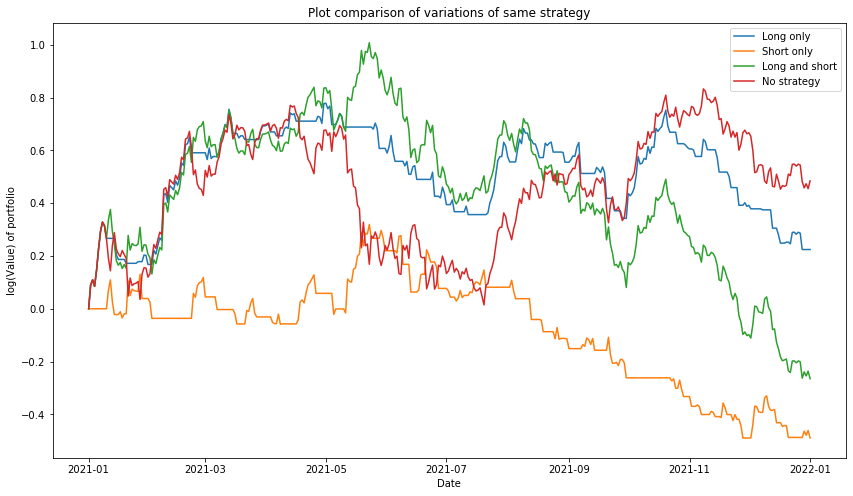
\includegraphics[width=1\linewidth]{images/trade_strat_performance.png}
    \caption{Performance of Heikin Ashi strategy over year 2021 for Bitcoin against US Dollars}
\end{figure}

\newpage

In addition, visualising the Heikin Ashi indicator itself reveals the way it changes over time for the same period.

\begin{figure}[H]
\centering
    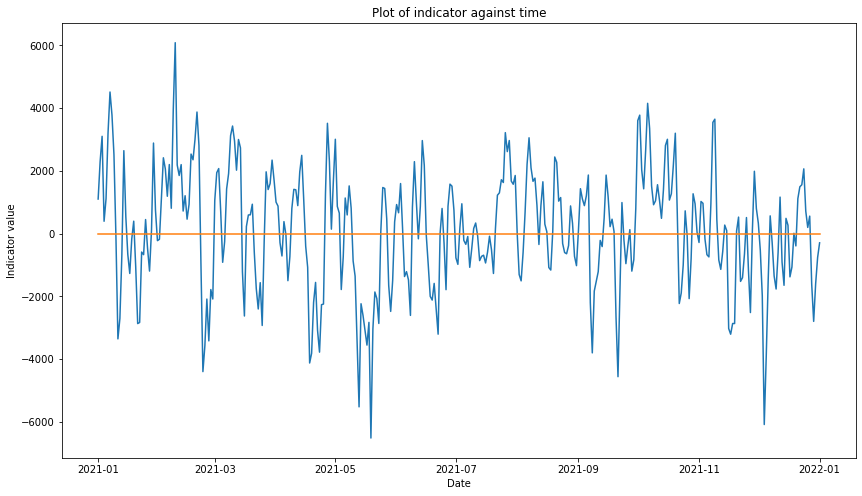
\includegraphics[width=1\linewidth]{images/indicator_graph.png}
    \caption{Heikin Ashi indicator series over year 2021 for Bitcoin against US Dollars}
\end{figure}

Evidently, following the Heikin Ashi indicator when trading Bitcoin was not a profitable strategy in 2021. This does not necessarily mean that Heikin Ashi under-performed for other assets.

\section{Bibliography}
\begin{enumerate}
    \item R. Velu, M. Hardy, D Nehren, (2020), Algorithmic Trading and Quantitative Strategies, CRC Press, Taylor \& Francis Group
    \item A. Cartea, S. Jaimungal, J. Penalva, (2015), Algorithmic and High Frequency Trading, Cambridge University Press
    \item M. J. Best, (2010), Portfolio Optimisation, CRC Press, Taylor \& Francis Group
    \item \texttt{https://www.investopedia.com/trading/heikin-ashi-better-candlestick/}
    \item \texttt{https://finance.yahoo.com/}
\end{enumerate}


\end{document}

